% A1 Decoupled PID with cross-coupling and back-EMF feedforward.
% Compile: pdflatex current-loop-a1-feedforward.tex && pdf2svg ...
\documentclass[tikz, margin=4mm]{standalone}
\usetikzlibrary{arrows.meta, positioning, calc}

\tikzset{
  block/.style = {draw, rectangle, rounded corners=2pt, align=center,
                  fill=blue!8, font=\small,
                  minimum height=1.0cm, minimum width=2.6cm},
  sum/.style   = {draw, circle, fill=blue!8, minimum size=7mm, inner sep=0pt},
  arr/.style   = {-{Latex[length=4pt, width=5pt]}, thick},
  lbl/.style   = {font=\footnotesize},
  node distance = 0.9cm and 1.6cm
}

\begin{document}
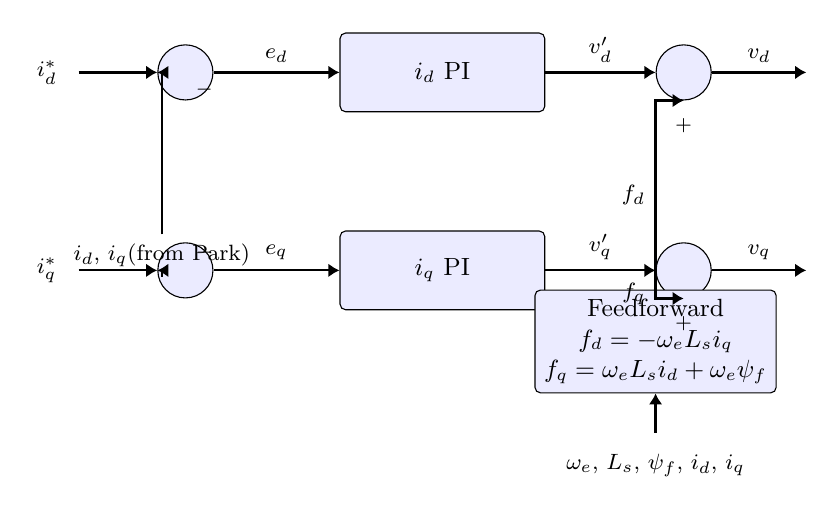
\begin{tikzpicture}

  % ── d-axis (top row) ──────────────────────────────────────────────────────
  \node[sum]                           (Sd)   {};
  \node[block, right=1.6cm of Sd]      (Pd)   {$i_d$ PI};
  \node[sum,   right=1.4cm of Pd]      (FFd)  {};   % feedforward summing

  % ── q-axis (bottom row) ───────────────────────────────────────────────────
  \node[sum,   below=1.8cm of Sd]      (Sq)   {};
  \node[block, right=1.6cm of Sq]      (Pq)   {$i_q$ PI};
  \node[sum,   right=1.4cm of Pq]      (FFq)  {};

  % ── Feedforward computation block ─────────────────────────────────────────
  \node[block, below=1.5cm of $(Pd.east)!0.5!(Pq.east)$, xshift=1.4cm]
        (FF) {Feedforward\\ $f_d = -\omega_e L_s i_q$\\ $f_q = \omega_e L_s i_d + \omega_e\psi_f$};

  % ── Output labels ─────────────────────────────────────────────────────────
  \coordinate (Vd_out) at ($(FFd.east)+(1.2,0)$);
  \coordinate (Vq_out) at ($(FFq.east)+(1.2,0)$);

  % ── I/O coordinates ───────────────────────────────────────────────────────
  \coordinate (IdRef) at ($(Sd.west)+(-1.0,0)$);
  \coordinate (IqRef) at ($(Sq.west)+(-1.0,0)$);
  % Feedback connections (id, iq from Park transform)
  \coordinate (FbTop) at ($(Sd.south)+(0,-0.3)$);  % below Sd
  \coordinate (FbBot) at ($(Sq.north)+(0, 0.3)$);  % above Sq

  % ── FF parameter inputs ───────────────────────────────────────────────────
  \coordinate (FFin)  at ($(FF.south)+(0,-0.5)$);

  % ── Connections ───────────────────────────────────────────────────────────

  % References
  \node[lbl, left=0.15cm of IdRef] {$i_d^*$};
  \node[lbl, left=0.15cm of IqRef] {$i_q^*$};
  \draw[arr] (IdRef) -- (Sd);
  \draw[arr] (IqRef) -- (Sq);

  % PIDs
  \draw[arr] (Sd)  -- node[lbl,above]{$e_d$} (Pd);
  \draw[arr] (Sq)  -- node[lbl,above]{$e_q$} (Pq);
  \draw[arr] (Pd)  -- node[lbl,above]{$v_d'$} (FFd);
  \draw[arr] (Pq)  -- node[lbl,above]{$v_q'$} (FFq);

  % Outputs
  \draw[arr] (FFd.east) -- node[lbl,above]{$v_d$} (Vd_out);
  \draw[arr] (FFq.east) -- node[lbl,above]{$v_q$} (Vq_out);

  % id, iq feedback to summing junctions (negative)
  \coordinate (id_fb) at ($(Sd.south)+(0,-0.5)$);
  \coordinate (iq_fb) at ($(Sq.south)+(0,-0.5)$);
  \node[lbl, below=0.8cm of $(Sd)!0.5!(Sq)$, xshift=-0.3cm] (IdIq) {$i_d,\,i_q$\\ (from Park)};
  \draw[arr] (IdIq.north) |- (Sd) node[below right, font=\scriptsize]{$-$};
  \draw[arr] (IdIq.south) |- (Sq) node[above right, font=\scriptsize]{$-$};

  % Feedforward block → summing junctions
  \draw[arr] (FF.north) |- node[lbl, left, pos=0.25]{$f_d$} (FFd.south);
  \draw[arr] (FF.north) |- node[lbl, left, pos=0.25]{$f_q$} (FFq.south);
  % Label the + signs on feedforward inputs
  \node[font=\scriptsize, below=0.1cm of FFd] {$+$};
  \node[font=\scriptsize, below=0.1cm of FFq] {$+$};

  % Parameter input to feedforward block
  \node[lbl, below=0.15cm of FFin] {$\omega_e,\,L_s,\,\psi_f,\,i_d,\,i_q$};
  \draw[arr] (FFin) -- (FF.south);

\end{tikzpicture}
\end{document}
